\chapter{Réalisation de la plateforme de données}
\label{ch:realisation}

\section{Mise en place du système source}

La sauvegarde \texttt{WideWorldImporters-Full.bak} (121 Mo) a été restaurée sur une instance locale de
SQL Server 2025 Developer. Deux obstacles ont été rencontrés :
\begin{itemize}
  \item le service SQL Server, exécuté sous un compte de service, n'avait pas le droit de lire le dossier
        \emph{Téléchargements} de l'utilisateur (« \emph{Operating system error 5 : Accès refusé} ») :
        la sauvegarde a été copiée dans un dossier partagé (\texttt{C:\textbackslash
        Users\textbackslash Public\textbackslash SQLBackups}) ;
  \item le pilote ODBC 18 chiffre les connexions par défaut et refusait le certificat auto-signé de
        l'instance locale : l'option \texttt{-C} (\texttt{TrustServerCertificate}) a été ajoutée.
\end{itemize}
La restauration a converti la base au format interne de SQL Server 2025 (version 852 vers 998) et a
produit 31 tables métier (hors tables d'archive).

\section{Ingestion dans la couche Bronze avec DLT}
\label{sec:bronze}

\subsection{Stratégie de chargement}
Le pipeline \texttt{ingestion/wwi\_pipeline.py} déclare une ressource DLT par table source. La
stratégie est choisie automatiquement à partir des métadonnées de chaque table
(tableau~\ref{tab:strategie}).

\begin{table}[H]
\centering
\caption{Stratégie de chargement par type de table}
\label{tab:strategie}
\begin{tabularx}{\linewidth}{@{}X l l r@{}}
\toprule
\textbf{Cas} & \textbf{Curseur} & \textbf{Écriture} & \textbf{Tables} \\
\midrule
Table transactionnelle avec \texttt{LastEditedWhen} et clé primaire & \texttt{LastEditedWhen} & \texttt{merge} & 12 \\
Table temporelle avec \texttt{ValidFrom} et clé primaire & \texttt{ValidFrom} & \texttt{merge} & 16 \\
Table d'archive (sans clé primaire) & --- & \texttt{replace} & 2 \\
\bottomrule
\end{tabularx}
\end{table}

En mode incrémental, DLT mémorise la plus grande valeur du curseur déjà chargée et n'extrait au passage
suivant que les lignes plus récentes ; ces lignes sont ensuite \textbf{fusionnées} sur la clé primaire,
ce qui met à jour les lignes modifiées sans créer de doublons.

\begin{lstlisting}[language=Python, caption={Choix automatique de la stratégie de chargement (extrait)}, label=lst:dlt]
for full_name in tables:
    schema, name = full_name.split(".")
    columns = {c["name"] for c in inspector.get_columns(name, schema=schema)}
    pk = inspector.get_pk_constraint(name, schema=schema)["constrained_columns"]
    # Incrémental uniquement avec une clé de fusion : sans clé, un "replace"
    # incrémental écraserait la table avec les seules nouvelles lignes
    cursor = next((c for c in CURSOR_COLUMNS if c in columns), None) if pk else None

    resource = sql_table(
        credentials=engine, table=name, schema=schema,
        backend="pyarrow", reflection_level="full",
        table_adapter_callback=drop_unsupported_columns,
        incremental=dlt.sources.incremental(cursor) if cursor else None,
    ).with_name(f"{schema}_{name}")
    if cursor:
        resource.apply_hints(write_disposition="merge", primary_key=pk)
    else:
        resource.apply_hints(write_disposition="replace")
    yield resource
\end{lstlisting}

\subsection{Traitements particuliers}
\begin{itemize}
  \item \textbf{Types non supportés} : les colonnes \texttt{geography} (localisations, frontières) et
        \texttt{varbinary} (photos, mots de passe hachés) sont retirées avant l'extraction par une
        fonction de rappel (\texttt{table\_adapter\_callback}). Elles n'ont pas d'usage analytique et
        certaines sont sensibles.
  \item \textbf{Performance} : l'extraction utilise le moteur \texttt{pyarrow}, qui transfère les
        données par blocs colonnes et les charge dans Snowflake au format Parquet.
  \item \textbf{Connexions} : DLT extrayant plusieurs tables en parallèle, le pool de connexions
        SQLAlchemy par défaut (5 + 10) était épuisé ; il a été remplacé par un \texttt{NullPool}.
\end{itemize}

\subsection{Résultat et réconciliation}
Le premier chargement complet transfère \textbf{30 tables} (près d'un million de lignes) en
environ une minute. Le script \texttt{ingestion/check\_bronze.py} compare, table par table, le nombre de lignes
entre SQL Server et Snowflake : les 28 tables principales présentent un écart nul. Une seconde exécution
n'extrait aucune ligne pour les tables incrémentales, ce qui confirme le bon fonctionnement du curseur.

\begin{table}[H]
\centering
\caption{Volumes des principales tables Bronze (réconciliées avec SQL Server)}
\label{tab:bronze}
\small
\begin{tabular}{@{}l r l r@{}}
\toprule
\textbf{Table} & \textbf{Lignes} & \textbf{Table} & \textbf{Lignes} \\
\midrule
\texttt{warehouse\_stock\_item\_transactions} & 236\,667 & \texttt{application\_cities} & 37\,940 \\
\texttt{sales\_order\_lines} & 231\,412 & \texttt{purchasing\_purchase\_order\_lines} & 8\,367 \\
\texttt{sales\_invoice\_lines} & 228\,265 & \texttt{purchasing\_supplier\_transactions} & 2\,438 \\
\texttt{sales\_customer\_transactions} & 97\,147 & \texttt{purchasing\_purchase\_orders} & 2\,074 \\
\texttt{sales\_orders} & 73\,595 & \texttt{application\_people} & 1\,111 \\
\texttt{sales\_invoices} & 70\,510 & \texttt{sales\_customers} & 663 \\
\bottomrule
\end{tabular}
\end{table}

\section{Couche Silver : nettoyage et normalisation}
\label{sec:silver}

La couche Silver compte \textbf{29 modèles dbt}. Les règles de nettoyage sont factorisées dans des
macros réutilisables (listing~\ref{lst:macros}) et appliquées de manière homogène à toutes les tables.

\begin{lstlisting}[language=SQL, caption={Macros de nettoyage (\texttt{macros/cleaning.sql}, extrait)}, label=lst:macros]
{# Texte nettoyé : espaces supprimés, chaînes vides -> NULL #}
{% macro clean_text(col) -%}
    nullif(trim({{ col }}), '')
{%- endmacro %}

{# Montant normalisé en décimal à 2 chiffres #}
{% macro to_amount(col) -%}
    cast({{ col }} as number(18, 2))
{%- endmacro %}

{# Dédoublonnage de sécurité : garde la version la plus récente par clé #}
{% macro dedup(key, order_col) -%}
    qualify row_number() over (partition by {{ key }} order by {{ order_col }} desc) = 1
{%- endmacro %}
\end{lstlisting}

\begin{table}[H]
\centering
\caption{Règles appliquées dans la couche Silver}
\label{tab:silver}
\begin{tabularx}{\linewidth}{@{}l X@{}}
\toprule
\textbf{Règle} & \textbf{Mise en œuvre} \\
\midrule
Texte & Suppression des espaces, chaînes vides converties en \texttt{NULL}, e-mails et URL en minuscules,
        codes ISO en majuscules \\
Montants & Conversion en \texttt{NUMBER(18,2)} ; taux en \texttt{NUMBER(5,3)} \\
Valeurs manquantes & Booléens à \texttt{false}, quantités à 0 \\
Dédoublonnage & Version la plus récente par clé (\texttt{QUALIFY ROW\_NUMBER()}) \\
Règles métier & Montant HT $=$ quantité $\times$ prix unitaire ; montant TTC $=$ \texttt{extended\_price} \\
Données semi-structurées & Pays de fabrication extrait du JSON \texttt{CustomFields} (\texttt{TRY\_PARSE\_JSON}) \\
Minimisation & Coordonnées bancaires des fournisseurs, identifiants de connexion et préférences des
               utilisateurs exclus \\
\bottomrule
\end{tabularx}
\end{table}

\section{Couche Gold : le schéma en étoile}

La couche Gold contient \textbf{15 tables} : 6 dimensions, 6 faits et 3 tables d'historisation
(tableau~\ref{tab:gold}).

\begin{table}[H]
\centering
\caption{Tables de la couche Gold}
\label{tab:gold}
\begin{tabularx}{\linewidth}{@{}l X r@{}}
\toprule
\textbf{Table} & \textbf{Grain et contenu} & \textbf{Lignes} \\
\midrule
\texttt{fact\_sales} & Ligne de facture : CA HT, TVA, TTC, bénéfice, quantité & 228\,265 \\
\texttt{fact\_orders} & Ligne de commande : quantités commandées et préparées, reliquats & 231\,412 \\
\texttt{fact\_purchases} & Ligne de bon de commande fournisseur : quantités et montants d'achat & 8\,367 \\
\texttt{fact\_customer\_transactions} & Transaction client : facture ou paiement, solde dû & 97\,147 \\
\texttt{fact\_stock\_movements} & Mouvement de stock : entrée ou sortie & 236\,667 \\
\texttt{fact\_stock\_holdings} & Produit : stock actuel, valeur, alerte de réapprovisionnement & 227 \\
\midrule
\texttt{dim\_date} & Jour (2013--2016), libellés français & 1\,461 \\
\texttt{dim\_customer} & Client : catégorie, groupement d'achat, territoire, pays & 663 \\
\texttt{dim\_product} & Produit : marque, couleur, groupe, fournisseur & 227 \\
\texttt{dim\_supplier} & Fournisseur : catégorie, pays, délai de paiement & 13 \\
\texttt{dim\_employee} & Employé, dont commerciaux & 19 \\
\texttt{dim\_city} & Ville, province, territoire commercial, pays, continent & 37\,940 \\
\midrule
\texttt{dim\_product\_history} & Version d'un produit (SCD2) : évolution des prix & 671 \\
\texttt{dim\_customer\_history} & Version d'un client (SCD2) : crédit, catégorie, remise & 713 \\
\texttt{fact\_stock\_history} & Version du niveau de stock (snapshot dbt) & 227+ \\
\bottomrule
\end{tabularx}
\end{table}

Le listing~\ref{lst:factsales} montre la construction de la table de faits des ventes, matérialisée de
manière incrémentale (section~\ref{sec:incremental}).

\begin{lstlisting}[language=SQL, caption={Table de faits des ventes (\texttt{fact\_sales.sql}, extrait)}, label=lst:factsales]
{{ config(materialized='incremental', unique_key='invoice_line_id',
          incremental_strategy='merge', on_schema_change='append_new_columns') }}

-- Grain : une ligne de facture
select
    il.invoice_line_id, il.invoice_id, i.order_id, i.invoice_date,
    i.customer_id, il.stock_item_id, i.salesperson_person_id as salesperson_id,
    c.delivery_city_id, dm.delivery_method_name as delivery_method,
    i.is_credit_note, il.quantity, il.unit_price, il.tax_rate,
    il.amount_excluding_tax, il.tax_amount, il.amount_including_tax,
    il.line_profit as profit,
    greatest(il.last_edited_when, i.last_edited_when) as last_edited_when
from {{ ref('slv_invoice_lines') }} il
join {{ ref('slv_invoices') }} i on i.invoice_id = il.invoice_id
left join {{ ref('slv_customers') }} c on c.customer_id = i.customer_id
left join {{ ref('slv_delivery_methods') }} dm on dm.delivery_method_id = i.delivery_method_id
{% if is_incremental() %}
where greatest(il.last_edited_when, i.last_edited_when) >
      (select coalesce(max(last_edited_when), '1900-01-01'::timestamp_ntz) from {{ this }})
{% endif %}
\end{lstlisting}

Une macro \texttt{generate\_schema\_name} redéfinit le comportement par défaut de dbt afin que les modèles
soient créés directement dans les schémas \texttt{SILVER} et \texttt{GOLD}, et une configuration
\texttt{grants} accorde automatiquement le droit \texttt{SELECT} sur toute table Gold au rôle
\texttt{WWI\_ANALYST}.

\section{Historisation des données (SCD de type 2)}
\label{sec:scd2}

La couche Bronze ne conserve que la dernière version de chaque ligne. Pour analyser l'évolution des
données dans le temps, deux mécanismes complémentaires ont été mis en place.

\subsection{Exploitation des tables temporelles de SQL Server}
Les tables temporelles de WWI conservent chaque version passée dans une table d'archive.
\texttt{Sales.Customers\_Archive} et \texttt{Warehouse.StockItems\_Archive} sont donc ingérées en Bronze,
puis réunies avec la version courante dans les modèles \texttt{slv\_stock\_items\_history} et
\texttt{slv\_customers\_history}. Chaque version reçoit une clé de substitution (hachage MD5 de
l'identifiant et de la date de début de validité). Les tables Gold \texttt{dim\_product\_history}
(671 versions pour 227 produits) et \texttt{dim\_customer\_history} (713 versions pour 663 clients)
exposent la période de validité, un numéro de version et un indicateur de version courante. Il devient
alors possible de répondre à des questions comme « comment le prix de tel produit a-t-il évolué ? ».

\subsection{Snapshot dbt du niveau de stock}
La table des niveaux de stock (\texttt{StockItemHoldings}) n'est pas temporelle : la source n'en garde
que la valeur courante. Un \textbf{snapshot dbt} (stratégie \texttt{check} sur la quantité, le coût,
le seuil et la cible de stock) enregistre une nouvelle version à chaque changement détecté lors d'une
exécution ; la table \texttt{fact\_stock\_history} en est issue. L'historique s'enrichit ainsi
automatiquement à chaque exécution quotidienne de la plateforme.

\begin{lstlisting}[language=yaml, caption={Snapshot dbt du niveau de stock (\texttt{snapshots.yml})}, label=lst:snapshot]
snapshots:
  - name: snp_stock_item_holdings
    relation: ref('slv_stock_item_holdings')
    config:
      schema: SILVER
      unique_key: stock_item_id
      strategy: check
      check_cols: [quantity_on_hand, last_cost_price, reorder_level, target_stock_level]
      hard_deletes: invalidate
\end{lstlisting}

\section{Qualité des données}

dbt exécute plus de \textbf{140 tests} à chaque construction (tableau~\ref{tab:tests}).

\begin{table}[H]
\centering
\caption{Typologie des tests de qualité}
\label{tab:tests}
\begin{tabularx}{\linewidth}{@{}l X@{}}
\toprule
\textbf{Type de test} & \textbf{Exemples} \\
\midrule
Unicité, non-nullité & Clé de chaque table Silver et Gold, clés de version SCD2 \\
Intégrité référentielle & Chaque fait pointe vers un client, un produit, une date, un employé existant \\
Valeurs autorisées & \texttt{direction} $\in$ \{Entrée, Sortie\} \\
Règles métier & HT $+$ TVA $=$ TTC (tolérance d'un centime) ; quantités vendues strictement positives ;
                dates de vente couvertes par \texttt{dim\_date} \\
Historisation & Exactement une version courante par produit et par client \\
Réconciliation & CA TTC de la couche Gold égal à celui de la couche Bronze \\
\bottomrule
\end{tabularx}
\end{table}

\begin{lstlisting}[language=SQL, caption={Test de réconciliation Bronze / Gold}, label=lst:test]
-- Réconciliation : le CA TTC de la couche Gold égale celui de la couche Bronze
with bronze as (
    select sum(extended_price) as total from {{ source('bronze', 'sales_invoice_lines') }}
),
gold as (
    select sum(amount_including_tax) as total from {{ ref('fact_sales') }}
)
select bronze.total as bronze_total, gold.total as gold_total
from bronze, gold
where abs(bronze.total - gold.total) > 1
\end{lstlisting}

Un test dbt échoue s'il renvoie au moins une ligne. La commande \texttt{dbt build} exécute les modèles
et leurs tests dans l'ordre des dépendances : un modèle dont un test échoue bloque ses descendants.

\section{Orchestration avec Dagster}

\subsection{Assets et lignage}
Le fichier \texttt{orchestration/definitions.py} déclare :
\begin{itemize}
  \item les \textbf{assets Bronze} à partir de la source DLT (\texttt{@dlt\_assets}) ; un traducteur
        personnalisé leur attribue la clé \texttt{["bronze", <table>]}, identique à celle des
        \emph{sources} dbt, ce qui relie automatiquement DLT et dbt dans le lignage ;
  \item les \textbf{assets Silver et Gold} à partir du manifeste dbt (\texttt{@dbt\_assets}), regroupés
        par couche ;
  \item les \textbf{tests dbt}, convertis automatiquement en \emph{asset checks}.
\end{itemize}

Au total, Dagster gère \textbf{75 assets} (30 Bronze, 30 Silver, 15 Gold) et \textbf{146 contrôles}
de qualité. La figure~\ref{fig:lineage} montre le lignage de la table \texttt{fact\_sales} : on y
retrouve les tables Bronze chargées par DLT, les modèles Silver et le fait Gold.

\begin{figure}[H]
\centering
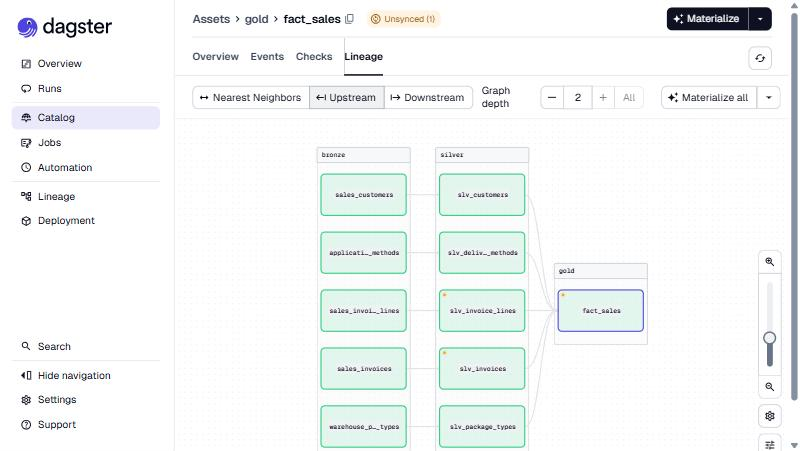
\includegraphics[width=0.92\linewidth]{figures/dagster_lineage.jpg}
\caption{Lignage amont de \texttt{gold/fact\_sales} dans Dagster (Bronze $\rightarrow$ Silver $\rightarrow$ Gold)}
\label{fig:lineage}
\end{figure}

\subsection{Planification et reprise sur erreur}
Le job \texttt{wwi\_daily\_job} rejoue toute la chaîne : ingestion DLT, puis \texttt{dbt build}. Il est
déclenché \textbf{chaque jour à 06\,h\,00 (heure de Dakar)} par le planning
\texttt{wwi\_daily\_schedule}. Une politique de reprise (\texttt{RetryPolicy}) relance automatiquement
une étape en échec jusqu'à deux fois, à 60 secondes d'intervalle, ce qui absorbe les erreurs
transitoires (réseau, verrou temporaire).

\begin{figure}[H]
\centering
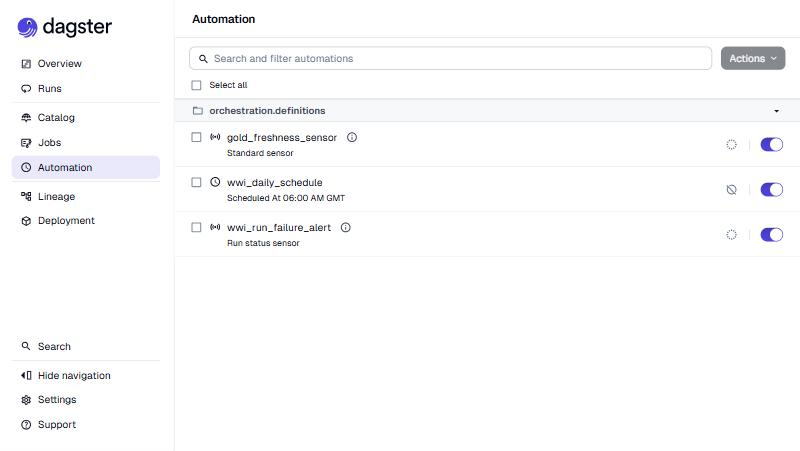
\includegraphics[width=0.85\linewidth]{figures/dagster_automation.jpg}
\caption{Automatisations actives dans Dagster : planning quotidien et capteurs d'alerte}
\label{fig:automation}
\end{figure}

Le premier run complet du job a réussi en environ 4\,min\,30 (3\,min\,32 pour l'étape Bronze, 53 s
pour l'étape dbt).
